\section{Experiments}
\label{sec:experiments}

This section evaluates the proposed method when applied to the drilling task
shown in \fref{fig:setup}. Our system is formed by a Denso VS060 6-\ac{dof}
industrial manipulator equipped with a commercial off-the-shelf hand drill. All
benchmarks were executed in a system with Intel\textsuperscript{\textregistered}
Core\texttrademark~i7 processor and 24 GB RAM, GeForce GTX 960M video card,
running Ubuntu 16.04 (Xenial), 64 bits.

\subsection{Benchmarking task-space \ac{tsp} solvers}
\label{sec:tsp_comparison}

To solve the task-space \ac{tsp} (Step~1 of our algorithm), one may use exact or
near-optimal solvers. The choice depends on the trade-off between the available
CPU time and the solution quality. Here we evaluate three \ac{tsp} solvers.

\begin{enumerate}

  \item \textit{Exact}: \ac{cip} can be used to find true optimal \ac{tsp}
  tour~\cite{Applegate2011}. Here, we used the \acs{scip} Optimization Suite
  \cite{Achterberg2009} to implement an exact solver;

  \item \textit{2-Opt}: We re-implemented this simple, yet efficient, algorithm
  to find a near-optimal solution to \ac{tsp}. The algorithm iteratively
  improves an initial guess by repeatedly replacing pairs of edges that cross
  over \cite{Applegate2011}.

  \item \textit{RNN}: We re-implemented this algorithm, which consists in
  iteratively selecting the nearest neighbor as the next target to visit. This
  process is repeated until all the targets are visited \cite{Applegate2011}.
  One can do several \emph{restarts} from different initial targets, and choose
  the tour with the lowest cost from all the restarts. The drawback of this
  method is that it tends to corner itself, which requires long edges to get
  back to unvisited targets.

\end{enumerate}

\begin{figure}[t]
  \centering
  \vspace*{2mm}
  \subfloat[]{\includegraphics[height=40mm]{tsp_solvers_times}}\;
  \subfloat[]{\includegraphics[height=40mm]{tsp_solvers_errors}}
  \caption{Benchmarking results for three task-space \ac{tsp} solvers. (a) CPU
  times for different number of targets. The Y axis is logarithmic (b) Task
  execution time for different number of targets. The sets of targets are
  selected randomly. The last sample considers all the $245$ targets.}
  \label{fig:tsp_solvers}
\end{figure}

\fref{fig:tsp_solvers} shows a benchmark of the three methods. We run the
\ac{tsp} solvers on task-space subsets of $25$, $50$, $100$, $150$, $200$ random
targets as well as on the total $245$ targets.  One can observe that the
\textit{2-Opt} solver yields high-quality tours (less than $5\%$ of
sub-optimality) with low CPU time usage (less than $1$\,s). As for the
\textit{Exact} solver, it is not practical for more than $150$ targets.
Therefore, for all the subsequent experiments, we shall use \textit{2-Opt} as
our near-optimal task-space \ac{tsp} solver.

\subsection{Benchmarking configuration-space metrics}
\label{sub:metrics_benchmark}

The \textit{configuration-space metric} that defines the edge cost in Step~2 of
our algorithm is the key component for the overall performance of the method.
Given two robot configurations $\vb*{q}$ and $\vb*{q}'$, the ideal cost of the
edge $c^{*}\qty(\vb*{q}, \vb*{q}')$ is the duration of a time-optimal
collision-free trajectory between them. However, since there are thousands of
such edges, running full-fledged motion planning algorithms (with collision
checks) for every edge would not be tractable. Therefore, one must consider
approximate metrics, which should be fast to compute, yet give a good prediction
of the corresponding time-optimal collision-free trajectory duration. Here we
evaluate three such metrics.

\begin{enumerate}

  \item \textit{Weighted Euclidean joint distance}: The cost $c\qty(\vb*{q},
  \vb*{q}')$ is estimated as the weighted $\mbox{L}^{2}$ norm:
  \begin{equation*}
    c\qty(\vb*{q}, \vb*{q}') :=
    \sqrt{\sum_{k=1}^{\mdof}w_{k}\qty(q'_{k}-q_{k})^2}\; ,
  \end{equation*}
  where $w_{k}$ is a positive weight for joint $k$. The weights are chosen in
  proportion to the maximum possible distance (Euclidean distance in the
  task-space) traveled by any point on the robot, when moving along the
  corresponding joint. Similar to \cite{Bohlin2000}, in our experiments this
  metric outperforms consistently the Euclidean joint distance.

  \item \textit{Maximum joint difference}: The cost $c\qty(\vb*{q}, \vb*{q}')$
  is estimated as follows:
  \begin{equation*}
    c\qty(\vb*{q}, \vb*{q}') :=
          \max_{k}\abs{\frac{\qty(q'_{k}-q_{k})}{\dot{q}_k}}\; .
  \end{equation*}
  The intuition of this metric is to determine the maximum joint displacement
  when \enquote{moving} from $\vb*{q}$ to $\vb*{q}'$ by simply computing the
  joint difference, $\qty(q'_{k}-q_{k})$, over the joint $k$ velocity limit, for
  $k \in \qty[1,\dots,\mdof]$. Then the maximum value is used;

  \item \textit{Linear trajectory interpolation}: the cost $c\qty(\vb*{q},
  \vb*{q}')$ is given by the duration of a trajectory obtained by linear
  interpolation. It only requires to specify the positions, $\vb*{q}$ and
  $\vb*{q}'$, and guarantees continuity at the position level subject to the
  robot velocity and acceleration bounds. Moreover, this metric does not
  consider obstacles which greatly reduces its computing time.

\end{enumerate}

\begin{figure}[t]
  \centering
  \vspace*{2mm}
  \subfloat[]{\includegraphics[height=40mm]{metrics_times}}\;
  \subfloat[]{\includegraphics[height=40mm]{metrics_duration}}
  \caption{Benchmarking results for three C-space metrics. (a) CPU times for
  different number of targets. The Y axis is logarithmic (b) Task execution time
  for different number of targets. The sets of targets are selected randomly.
  The last sample considers all the $245$ targets.}
  \label{fig:metrics_benchmark}
\end{figure}

\fref{fig:metrics_benchmark} shows the benchmarking results for the
three proposed configuration-space metrics. One can observe that the
\textit{Maximum joint difference} metric takes the lowest CPU time and
yields task execution times comparable to, in some cases even better
than, the \textit{Euclidean} and \textit{Linear Interpolation
  metrics}. Therefore, for all the subsequent experiments, we shall
use \textit{Maximum joint difference} as our metric.

\subsection{Benchmarking discretization step size for the free \ac{dof}}
\label{sub:discrete_benchmark}

Many industrial tasks such as spot-welding, spay-painting or drilling involve
less than 6 degrees of freedom. Therefore, a classical 6-\ac{dof} industrial
robot has more joints than strictly required to execute such tasks.
Specifically, the drilling task at hand involves 5 \ac{dof}, since the rotation
$\theta$ about the drilling direction is irrelevant. One approach to tackle this
redundancy can consist in setting a specific value for the irrelevant \ac{dof}:
for instance $\theta \in \{0, \frac{\pi}{2}, \pi, \frac{3\pi}{2}\}$ for a
$\frac{\pi}{2}$ discretization step size. For each of the discretized value of
$\theta$, we then have a full 6-\ac{dof} \ac{ik} problem. To solve the full
6-\ac{dof} \ac{ik}, we next use OpenRAVE's IKFast \cite{diankov2010}, which
outputs all the \ac{ik} solutions (here we have a \enquote{discrete} redundancy
situation -- think of the \enquote{elbow up} and \enquote{elbow down}
configurations). We finally group all the IK solutions corresponding to all the
discretized values of $\theta$ into a single list, which is the list of all IK
solutions that will be considered for a given target. \tref{tab:discret_effect}
gives the total number of IK solutions considered as a function of the
discretization step size and of the number of targets.

\renewcommand{\arraystretch}{1.5}
\begin{table}[htp]
\caption{Number of robot configurations depending on the discretization
step size and the number of targets}
\label{tab:discret_effect}
\centering
\begin{tabular}{c c c c c c c}
\toprule
\textbf{Step} & \multicolumn{6}{c}{\textbf{Number of targets}}  \\
\textbf{Size} & \bm{$25$} & \bm{$50$}  & \bm{$100$} & \bm{$150$} & \bm{$200$} & \bm{$245$}\\
\midrule
$\pi$            & $209$   & $462$   & $1,049$ & $1,540$  & $2,059$  & $2,486$\\
$\frac{\pi}{2}$  & $329$   & $723$   & $1,569$ & $2,311$  & $3,100$  & $3,770$\\
$\frac{\pi}{3}$  & $452$   & $1,053$ & $2,231$ & $3,297$  & $4,425$  & $5,409$\\
\bm{$\frac{\pi}{4}$} & \bm{$630$} & \bm{$1,369$} & \bm{$2,850$} & \bm{$4,238$} & \bm{$5,727$} & \bm{$6,975$}\\
$\frac{\pi}{6}$  & $898$   & $2,011$ & $4,287$ & $6,363$  & $8,492$  & $10,406$\\
$\frac{\pi}{12}$ & $1,820$ & $4,038$ & $8,448$ & $12,605$ & $16,933$ & $20,693$\\
\bottomrule
\end{tabular}
\end{table}

One can see that the choice of the \textit{discretization step size} is governed
by a trade-off between speed and optimality. \fref{fig:discrete} shows the
computation time and task execution time as a function of the discretization
step size. As expected, the computation time increases as the discretization
step size decreases, but interestingly, the task execution time does not change
significantly for step sizes below $\frac{\pi}{4}$, which thus yields a good
trade-off between CPU time and task execution time. Therefore, for all the
subsequent experiments, we shall use $\frac{\pi}{4}$ as our discretization step
size.


\begin{figure}[t]
  \centering
  \vspace*{2mm}
  \subfloat[]{\includegraphics[height=40mm]{discrete_times}}\;
  \subfloat[]{\includegraphics[height=40mm]{discrete_duration}}
  \caption{Benchmarking results showing the effect of the discretization step size
  of the free \ac{dof}.}
  \label{fig:discrete}
\end{figure}

\subsection{Comparison to other methods}
\label{sub:other_methods}

As none of the methods described in \sref{sec:related} provide public
implementations, we were unable to reproduce their results and perform a fair
comparison with the method herein presented. However, we can note that the
computation times reported in previous works are several orders of magnitude
higher than ours, yet for problem instances that are smaller\,\footnote{The
problem instance size is considered in terms of targets and configurations per
target} than what we consider in this work.

In the following, we compare our method to two of the existing methods, which we
could re-implement.

\begin{enumerate}

  \item \textit{\acs{tsp} in C-space}~\cite{Edan1991}: when only one
  configuration is considered per target, \ac{rtsp} is reduced to a regular
  \ac{tsp} in the configuration space. Here, for each target, we consider the
  \ac{ik} solution with the best manipulability index~\cite{Yoshikawa1985};

  \item \textit{\acs{glkh}}: here the \ac{rtsp} is formulated as a
  \ac{gtsp}~\cite{Saha2006,Wurll1999,Wurll2001}. To solve that \ac{gtsp}, we use
  the state-of-the-art \acs{glkh} solver~\cite{Helsgaun2015} which makes use of
  the \ac{lkh} heuristic~\cite{Helsgaun2000}.

\end{enumerate}

\begin{figure}[t]
  \centering
  \subfloat{\includegraphics[height=40mm]{methods_times}}\;
  \subfloat{\includegraphics[height=40mm]{methods_cost}}  \\
  \subfloat{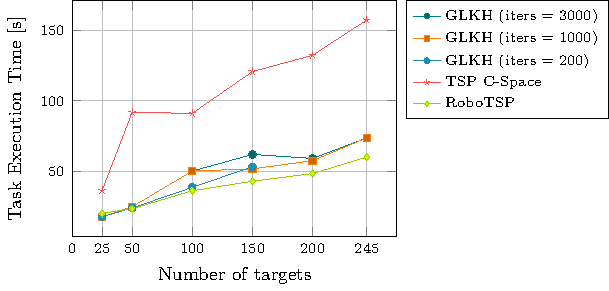
\includegraphics[height=40mm]{methods_duration}}
  \caption{Comparison of our method (\textit{RoboTSP}) against other methods: i)
  Solved as \acs{tsp} in configuration-space; ii) Solved as \acs{gtsp} using
  \acs{glkh}.}
  \label{fig:other_methods}
\end{figure}

\fref{fig:other_methods} shows the comparison of our method (\textit{RoboTSP})
to the two methods just described. While the \textit{\acs{tsp} in C-space}
method has a similar running time as \textit{RoboTSP} (indeed both run a
\ac{tsp} on the same number of targets), the time durations of the trajectories
it produces are higher than those of \textit{RoboTSP}, since it does not
optimize the \ac{ik} choice per target.

\textit{\acs{glkh}} produces trajectories with similar total duration as
\textit{RoboTSP} but the computing time is higher several orders of magnitude.

%%% Local Variables:
%%% mode: latex
%%% TeX-master: "../main"
%%% End:
